








\section{Proposed Method}
Inspired by recent advances in %data augmentation approaches in 
augmentation-based GCL, our approach learns node representations by rebalancing spectrum of two data views and performing the spectral feature augmentation via the incomplete power iteration. SFA is complementary to the existing data augmentation approaches.  Figure~\ref{fig:framework1} illustrates our framework. The \nameref{sec:not} section (supplementary material) explains our notations.

\vspace{0.1cm}
\noindent\textbf{Graph Augmentation ($\mathcal{A}_G$).}  
%Graph Augmentation 
%$\mathcal{A}_G$ 
Augmented graph $(\tilde{\mathbf{A}}, \tilde{\mathbf{X}})$ is generated by $\mathcal{A}_G$ by directly adding random perturbations to the original graph $({\mathbf{A}}, {\mathbf{X}})$.
%
Different augmented graphs are constructed given one input $(\mathbf {A}, \mathbf {X})$, yielding correlated views,  \ie, $(\widetilde{\mathbf{A}}^\alpha, \widetilde{\mathbf{X}}^\alpha)$ and $(\widetilde{\mathbf{A}}^\beta, \widetilde{\mathbf{X}}^\beta)$.
%
In the common GCL setting~\cite{zhu2020deep}, the graph structure is augmented by  permuting edges, whereas attributes by masking.
% \item

\vspace{0.1cm}
\noindent\textbf{Graph Neural Network Encoders.} 
Our framework admits various choices of the graph encoder. We opt for simplicity and adopt the commonly used graph convolution network (GCN)~\cite{kipf2016semi} as our base graph encoder. As shown in Fig.~\ref{fig:framework1}, we use a shared graph encoder for each view, \ie, $f: \mathbb{R}^{n \times d_{x}} \times \mathbb{R}^{n \times n}\longmapsto\mathbb{R}^{n \times d_{h}}$. We consider two graphs generated from $\mathcal{A}_G$  as two congruent structural views and define the GCN encoder with 2 layers as: 
 \begin{equation}
    \begin{aligned}
    &f(\mathbf{X}, \mathbf{A})=\mathrm{GCN}_{2}\left (\mathrm{GCN}_{1} (\mathbf{X}, \mathbf{A}), \mathbf{A}\right),\\
    &\quad\text{ where }\quad 
    \mathrm{GCN}_{l} (\mathbf{X}, \mathbf{A})=\sigma\big(\hat{\mathbf{D}}^{-\frac{1}{2}} \hat{\mathbf{A}} \hat{\mathbf{D}}^{-\frac{1}{2}} \mathbf{X} \Theta \big).
    \end{aligned}
\end{equation}
Moreover, $\tilde{\mathbf{A}}=\hat{\mathbf{D}}^{-1 / 2} \hat{\mathbf{A}} \hat{\mathbf{D}}^{-1 / 2} \in \mathbb{R}^{n \times n}$ is the degree-normalized adjacency matrix, $\hat{\mathbf{D}} \in \mathbb{R}^{n \times n}$ is the degree matrix of $\hat{\mathbf{A}}=\mathbf{A}+\mathbf{I}_{\mathbf{N}}$ where $\mathbf{I}_{\mathbf{N}}$ is the identity matrix, $\mathbf{X} \in \mathbb{R}^{n \times d_{x}}$ contains the initial node features, $\boldsymbol{\Theta} \in \mathbb{R}^{d_{x} \times d_{h}}$ contains network parameters, and $\sigma(\cdot)$ is a parametric ReLU (PReLU). % nonlinearity.
The encoder outputs feature maps $\mathbf{H}^\alpha$ and $\mathbf{H}^\beta$ for two views.
% \begin{algorithm}[tb]
%   \caption{Proposed Method}
% \begin{algorithmic}
%   \STATE {\bfseries Input:} Graph $(\mathbf{X},\mathbf{A})$, Graph augmentation $\mathcal{A}_{G}$; The number of iterations $k$.
%   \STATE $(\widetilde{\mathbf{X}}^\alpha, \widetilde{\mathbf{A}}^\alpha) = \mathcal{A}_G((\mathbf{X}, \mathbf{A}))$   \# \verb+Graph augmentation for view 1+
%   \STATE $(\widetilde{\mathbf{X}}^\beta, \widetilde{\mathbf{A}}^\beta) = \mathcal{A}_G((\mathbf{X}, \mathbf{A}))$   \# \verb+Graph augmentation for view 2+
%   \STATE $\mathbf{H}^\alpha = f(\widetilde{\mathbf{X}}^\alpha, \widetilde{\mathbf{A}}^\alpha)$
%   \STATE $\mathbf{H}^\beta = f(\widetilde{\mathbf{X}}^\beta, \widetilde{\mathbf{A}}^\beta)$
%   \STATE $\widetilde{\mathbf{H}}^\alpha = \mathcal{A}_F(\mathbf{H}^\alpha, k)$   \# \verb+Feature space augmentation for view 1+
%   \STATE $\widetilde{\mathbf{H}}^\beta = \mathcal{A}_F(\mathbf{H}^\beta, k)$    \# \verb+Feature space augmentation for view 2+
%   \STATE $\mathbf{Z}^\alpha = \theta(\widetilde{\mathbf{H}}^\alpha)$
%   \STATE $\mathbf{Z}^\beta = \theta(\widetilde{\mathbf{H}}^\beta)$
%   \STATE Compute $\mathcal{L}_{contrastive}$ for back propagation.
% %   \UNTIL{$noChange$ is $true$}
% % \STATE \textbf{Return} $\widetilde{\mathbf{H}}$
% \end{algorithmic}
% \label{algo:proposedMe}
% \end{algorithm}

\vspace{0.1cm}
\noindent\textbf{Spectral Feature Augmentation (SFA).}
$\mathbf{H}^\alpha$ and $\mathbf{H}^\beta$ are  fed to the feature augmenting function $\mathcal{A}_{F^*}$  where random noises are added to the spectrum via the incomplete power iteration. We explain the proposed SFA in the \nameref{sec:FA}~section and detail its properties in Propositions~\ref{prop:FeatureAug}, \ref{prop:PowerIter1} and \ref{prop:PowerIterVar}. SFA results in the spectrally-augmented feature maps, \ie, $\widetilde{\mathbf{H}}^\alpha$ and $\widetilde{\mathbf{H}}^\beta$. SFA is followed by a shared projection head $\theta: \mathbb{R}^{n \times d_{h}} \longmapsto \mathbb{R}^{n \times d_{z}}$ which is an MLP with two hidden layers and PReLU nonlinearity. It maps $\widetilde{\mathbf{H}}^\alpha$ and $\widetilde{\mathbf{H}}^\beta$ into  two node representations
$\mathbf{Z}^{\alpha}, \mathbf{Z}^{\beta} \in \mathbb{R}^{n \times d_{z}}$ (two congruent views of one graph) on which the contrastive loss is applied. As described in~\cite{chen2020simple}, it is beneficial to define the contrastive loss on $\mathbf{Z}$ rather than $\mathbf{H}$.

\vspace{0.1cm}
\noindent\textbf{Contrastive Training.}
To train the encoders end-to-end and learn rich node
 representations that are agnostic to downstream tasks, we utilize the InfoNCE loss~\cite{chen2020simple}: % which is defined as follows:
\begin{equation}
\label{equ:InfoNCE}
\begin{aligned}
&\mathcal{L}_{contrastive}(\tau)=\underbrace{\underset{\mathbf{z}, \mathbf{z}^{+}}{\mathbb{E}}\left[-\mathbf{z}^{\top} \mathbf{z}^{+}/\tau \right]}_{alignment}\\
&+ \underbrace{\underset{\mathbf{z}, \mathbf{z}^{+} %, \{\mathbf{z}_i^{-}\}_{i=1}^{2N-2}
}{\mathbb{E}}\Big[\log \Big(e^{{\mathbf{z}^\top\mathbf{z}^{+}}/{\tau}} \;\;+ \!\!\!\!\!\!\!\!\sum_{\mathbf{z}^{-} \in \mathbf{Z}^{\alpha\beta} \setminus \{\mathbf{z}, \
\mathbf{z}^{+}\}} \!\!\!\!\!\!\!\! e^{{\mathbf{z}^\top\mathbf{z}^{-}}/{\tau}}\Big)\Big]}_{uniformity},
\end{aligned}
\end{equation}
where $\mathbf{z}$ is the representation
of the anchor node in one view (\ie, $\mathbf{z} \in \mathbf{Z}^{\alpha}$) and $\mathbf{z}^{+}$ denotes the representation of the anchor node in another view (\ie,  $\mathbf{z}^{+} \in \mathbf{Z}^{\beta}$), whereas $\{\mathbf{z}^{-}\}$ are from the set of node representations other than $\mathbf{z}$ and $\mathbf{z}^{+}$ (\ie, $\mathbf{Z}^{\alpha\beta}\!\equiv\mathbf{Z}^\alpha \cup \mathbf{Z}^\beta$ and $\mathbf{z}^{-} \!\in \mathbf{Z}^{\alpha\beta}\setminus \{\mathbf{z}, \
\mathbf{z}^{+}\}$). The first part of  Eq.~\eqref{equ:InfoNCE} maximizes the alignment of two  views (representations of the same node become similar). The second part of  Eq.~\eqref{equ:InfoNCE} minimizes the pairwise similarity via LogSumExp. Pushing node representations away from each other  makes them uniformly distributed~\cite{wang2020understanding}. 
\begin{algorithm}[t]
% \begin{minpage}{0.45\textwidth}
% \resizebox{}{}{}
   \caption{Spectral Feature Augmentation ($\mathcal{A}_{F^*}$)}
\begin{algorithmic}
   \STATE {\bfseries Input:} feature map $\mathbf{H}$; the number of iterations $k$;
   \STATE $\mathbf{r}^{(0)} \sim \mathcal{N}(0, \mathbf{I})$
%   \REPEAT
%   \STATE Initialize $noChange = true$.
   \FOR{$i=1$ {\bfseries to} $k$}
%   \IF{$x_i > x_{i+1}$}
   \STATE $\mathbf{r}^{(i)} = \mathbf{H}^\top \mathbf{H} \mathbf{r}^{(i-1)}$
%   \STATE $noChange = false$
%   \ENDIF
   \ENDFOR
   \STATE $\widetilde{\mathbf{H}} = \mathbf{H} -  \frac{\mathbf{H} \mathbf{r}^{(k)} {\mathbf{r}^{(k)}}^{\top}}{\|\mathbf{r}^{(k)}\|_2^2}$ %where $\;\mathbf{r}= \mathbf{r}^{(k)}$
%   \UNTIL{$noChange$ is $true$}
\STATE \textbf{Return} $\widetilde{\mathbf{H}}$
\end{algorithmic}
\label{algo:1}
% \end{minpage}
\end{algorithm}
%
\subsection{Spectral Feature Augmentation for GCL}
\label{sec:FA}
\begin{figure*}[t]
    \vspace{-0.5cm}
    \centering
    \begin{subfigure}[b]{0.22\textwidth}
    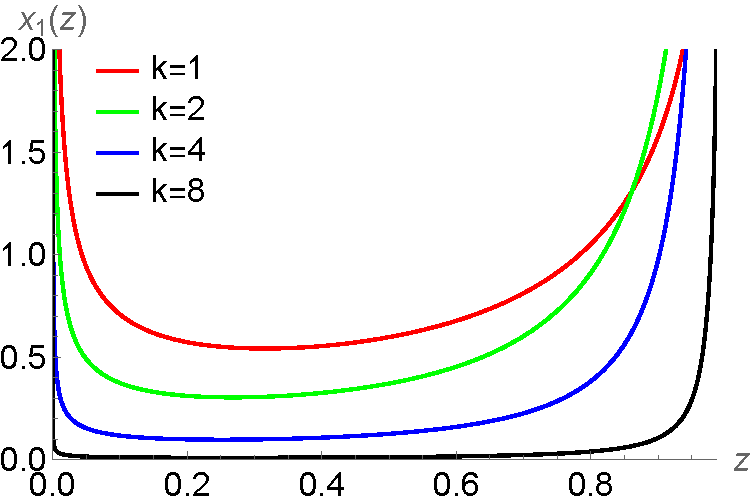
\includegraphics[width=\textwidth]{picture/sim_dist.pdf}
    \caption{\label{fig:sim1}  }
    \end{subfigure}
    \hspace{10px}
    \begin{subfigure}[b]{0.22\textwidth}
    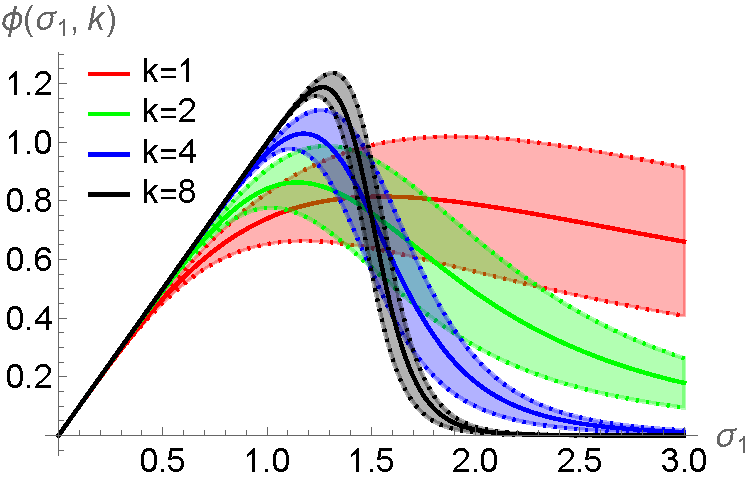
\includegraphics[width=\textwidth]{picture/sim_muvar.pdf}
    \caption{\label{fig:sim2}  }
    \end{subfigure}
     \hspace{10px}
    \begin{subfigure}[b]{0.22\textwidth}
    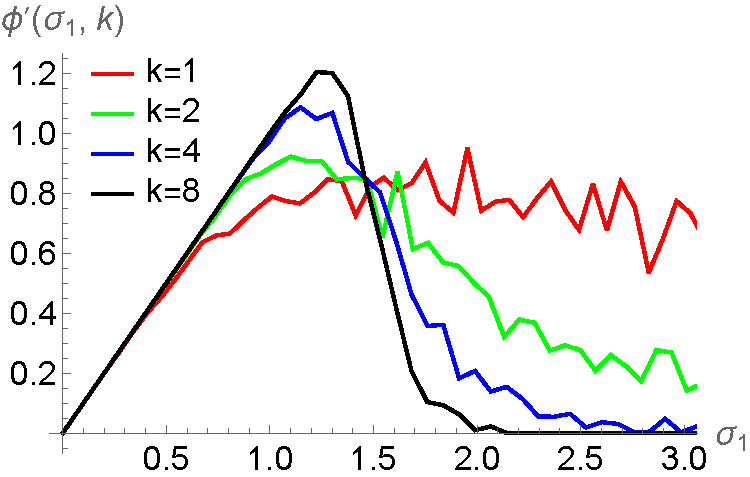
\includegraphics[width=\textwidth]{picture/sim_iter.pdf}
    \caption{\label{fig:sim3}  }
\end{subfigure}
%\begin{subfigure}[b]{0.24\textwidth}
%\includegraphics[width=\textwidth]{picture/pic4.pdf}
%\caption{\label{fig:sim4} }
%\end{subfigure}
\vspace{-0.2cm}
\caption{Toy illustration of Prop. \ref{prop:PowerIter1} and \ref{prop:PowerIterVar}. Let $\sigma_2,\cdots,\sigma_5$ be $1.5,0.9,0.2,0.01$. We investigate the impact of  iterations $k\in\{1,2,4,8\}$. Fig. \ref{fig:sim1} shows distribution $x(z)$ given $\sigma_1=2$. Fig.  \ref{fig:sim2} shows the expected value $\phi(\sigma_1,k)=\sigma_1(1-\lambda_1)$ where $\lambda_1=\mathbb{E}_{z\sim x_1}(z)$ for $0\leq\sigma_1\leq3$. The deviation is indicated by $\phi_{\pm\omega_1}(\sigma_1,k)=\sigma_1(1-\lambda_1\pm\omega_1)$. Finally, Fig. \ref{fig:sim3}  is obtained via Alg. \ref{algo:1} (the incomplete power iteration). To this end, we generated randomly a feature matrix $\mathbf{H}$ %, obtained its singular vector matrices $\mathbf{U}$ and $\mathbf{V}$, and then obtained  $\mathbf{H}'=\mathbf{U}\text{diag}(\sigma_1,\cdots, \sigma_{5})\mathbf{V}^\top$ by replacing singular values. 
%
and substituted its singular values by $\sigma_1,\cdots,\sigma_5$. Notice that for $k=1$, $1\leq\sigma_1\leq 3$, push-forward $\phi(\sigma_1,1)$ and $\phi'(\sigma_1,1)$ in Fig. \ref{fig:sim2} and \ref{fig:sim3} are around 0.8 (the balancing of spectrum) and the high deviation indicates the singular value undergoes  the spectral augmentation. For $k\geq 2$, both balancing and spectral augmentation effects decline. Note theoretical $\phi$ in Prop. \ref{prop:PowerIter1}  and real $\phi'$ from Alg. \ref{algo:1} match.
\label{fig:sim}
\vspace{-0.4cm}
}
\end{figure*}
Our spectral feature augmentation is inspired by the rank-1 update~\cite{yu2020toward}. %, and highlight various intuitions and theoretical insights. 
Let  $\mathbf{H} = f(\mathbf{X}, \mathbf{A})$ be the graph feature map with the singular decomposition  $\mathbf{H} = \mathbf{U}\mathbf{\Sigma}\mathbf{V}^\top$ where $\mathbf{H} \in \mathbb{R}^{n \times d_h}$,  $\mathbf{U}$ and $\mathbf{V}$ are unitary matrices, and $\mathbf{\Sigma} = \text{diag}(\sigma_1, \sigma_2,\cdots, \sigma_{d_h})$ is the diagonal matrix with  singular values $\sigma_1 \geq \sigma_2 \geq \cdots \geq \sigma_{d_h}$.
Starting from a random point $\mathbf{r}^{(0)} \sim \mathcal{N}(0,\mathbf{I})$ and  function $\mathbf{r}^{(k)} = \mathbf{H}^\top \mathbf{H} \mathbf{r}^{(k-1)}$,
we generate a set of augmented feature maps\footnote{We apply Eq. \eqref{equ:FeatureAug} on both views $\mathbf{H}^\alpha$ and $\mathbf{H}^\beta$ separately to obtain spectrally rebalanced/augmented  $\widetilde{\mathbf{H}}^\alpha$ and $\widetilde{\mathbf{H}}^\beta$.} $\widetilde{\mathbf{H}}$ by:
%

\vspace{-0.4cm}
\begin{equation}
\label{equ:FeatureAug}
    \widetilde{\mathbf{H}}\big(\mathbf{H}; \mathbf{r}^{(0)}\big) =\mathbf{H} - \mathbf{H}_{\text{LowRank}} =  \mathbf{H} - \frac{\mathbf{H} \mathbf{r}^{(k)} \mathbf{r}^{(k)\top}}{\|\mathbf{r}^{(k)}\|_2^2}.
\end{equation}
\vspace{-0.2cm}
%

\noindent 
We often write $\widetilde{\mathbf{H}}$ rather than $\widetilde{\mathbf{H}}\big(\mathbf{H}; \mathbf{r}^{(0)}\big)$, and we often think of  $\widetilde{\mathbf{H}}$ as a matrix. We summarize the proposed SFA in Alg.~\ref{algo:1}.
\begin{proposition}
\label{prop:FeatureAug}
Let $\widetilde{\mathbf{H}}$ be the augmented feature matrix obtained via Alg.~\ref{algo:1} for the $k$-th iteration starting from a random vector $\mathbf{r}^{(0)}$ drawn from $\mathcal{N}(0,\mathbf{I})$. Then $\,\mathbb{E}_{\mathbf{r}^{(0)}\sim \mathcal{N}(0,\mathbf{I})} (\widetilde{\mathbf{H}}\big(\mathbf{H}; \mathbf{r}^{(0)}\big))=\mathbf{U} \widetilde{\Sigma} \mathbf{V}^{\top}\!$ has rebalanced spectrum\footnote{$\,$``Rebalanced'' means the output spectrum is flatter than the input.$\!\!\!\!$} $\;\widetilde{\boldsymbol{\Sigma}} = \text{diag}\big[(1-\lambda_1(k)\sigma_1, (1-\lambda_2(k))\sigma_2, \cdots, (1-\lambda_{d_h}(k))\sigma_{d_h}\big]\;$ where $\lambda_i(k)=\mathbb{E}_{\mathbf{y}\sim\mathcal{N}(0;\mathbf{I})}\big(\frac{\left(y_{i} \sigma_{i}^{2k}\right)^{2}}{ \sum_{l=1}^{d_h}\left(y_{l} \sigma_{l}^{2k}\right)^{2}})$ and $\mathbf{y} = \mathbf{V}^{\top}\mathbf{r}^{(0)}$, because $0\leq 1-\lambda_1(k) \leq 1-\lambda_2(k) \leq \cdots \leq 1-\lambda_{d_h}(k)\leq 1\;$ for $\;\sigma_1 \geq \sigma_2 \geq \cdots \geq \sigma_{d_h}$ (sorted singular values from the SVD), and so $(1-\lambda_i)$ gets smaller or larger  as $\sigma_i$ gets larger or smaller, respectively.
\end{proposition}

% \begin{remark}
% Due to the power iteration, when $k\xrightarrow[]{} +\infty$, the series of $\mathbf{r}^{(k)}$ quickly converge to $\mathbf{v}_0$ the largest eigenvector of $\mathbf{H}^\top\mathbf{H}$. In this case 
% we have:
% \begin{equation}
%     \lim_{k\xrightarrow[]{} +\infty}\widetilde{\mathbf{H}} = \mathbf{U}\,\text{diag}(0, \sigma_2, \cdots, \sigma_{d_h})\mathbf{V}^\top.
% \end{equation}
% \end{remark}

%\definecolor{LightCyan}{rgb}{0.88,1,1}

\definecolor{beaublue}{rgb}{0.88,15,1}
\definecolor{blackish}{rgb}{0.2, 0.2, 0.2}
\begin{tcolorbox}[width=1.0\linewidth, colframe=blackish, colback=beaublue, boxsep=0mm, arc=2mm, left=2mm, right=2mm, top=2mm, bottom=2mm]
%\begin{tcolorbox}[colframe=black]
\noindent\textbf{Push-forward Function (\textit{Partial balancing of spectrum}).} Prop. \ref{prop:FeatureAug} shows that in expectation, our incomplete power iteration rebalances spectrum according to the push-forward function  $\phi(\sigma_i;k)=\sigma_i(1\!-\!\lambda_i(k))$ where $\lambda_i(k)$ is an expected value of $\lambda'_i(\mathbf{y},k)=\frac{\left(y_{i} \sigma_{i}^{2k}\right)^{2}}{ \sum_{l=1}^{d_h}\left(y_{l} \sigma_{l}^{2k}\right)^{2}}$ \wrt  random variable $\mathbf{y}\!\sim\!\mathcal{N}(0, \mathbf{I})$ (see Eq. \eqref{eq:balanceq}). 
\end{tcolorbox}

\definecolor{beaublue}{rgb}{0.88,15,1}
\definecolor{blackish}{rgb}{0.2, 0.2, 0.2}
\begin{tcolorbox}[width=1.0\linewidth, colframe=blackish, colback=beaublue, boxsep=0mm, arc=2mm, left=2mm, right=2mm, top=2mm, bottom=2mm]
%\vspace{0.1cm}
\textbf{Alg.~\ref{algo:1} returns an instance governed by the currently drawn $\mathbf{y}$}. The push-forward function in a feed-forward step of network realizes $\phi'(\sigma_i;\mathbf{y},k)=\sigma_i(1-\lambda'_i(\mathbf{y},k))$. Thus, below we study the analytical expression for $\phi(\sigma_i;k)$ and its variance to understand how drawing $\mathbf{y}\!\sim\!\mathcal{N}(0, \mathbf{I})$ translates into the variance posed by the implicit spectral augmentation of the singular values.
\end{tcolorbox}


%As Prop. \ref{prop:FeatureAug} merely indicates the balancing properties of the incomplete power iteration, the following two theorems study the analytical expected value and variance of .

\vspace{-0.1cm}
\begin{proposition}{{\em Analytical Expectation.}}
\label{prop:PowerIter1}
Let $\beta_i=(\sigma_i^{2k})^2$, then the expected value $\mathbb{E}_{\mathbf{y}\sim\mathcal{N}(0;\mathbf{I})}\frac{\beta_i y_{i}^2}{\beta_i y_{i}^2 +\sum_{l\neq i}\beta_l y^2_{l} } = \lambda_i(k)$ can be expressed as  $\mathbb{E}(x_i)$ over random variable $x_i\!=\!\frac{u}{u+v_i}$ for $u\!\sim\!\mathcal{G}(\frac{1}{2},2)$ and %$v\sim\Gamma\Big(\frac{1}{2}\frac{(\sum_{l\neq i}\beta_l)^2 }{\sum_{l\neq i}\beta_l^2}, \frac{2}{\beta_i}\frac{\sum_{l\neq i}\beta_l^2 }{\sum_{l\neq i}\beta_l}\Big)$
%
$v_i\!\sim\!\mathcal{G}(\alpha_i, 2\gamma_i)$ ($\mathcal{G}$ is Gamma distr.) with 
%
$\alpha_i\!=\!\frac{1}{2}\frac{(\sum_{l\neq i}\beta_l)^2 }{\sum_{l\neq i}\beta_l^2}$ and $\gamma_i\!=\!\frac{1}{\beta_i}\frac{\sum_{l\neq i}\beta_l^2 }{\sum_{l\neq i}\beta_l}$.
%
%
As PDF $x^\bullet_i(z)\!=\!\frac{\gamma_i}{(1-(1-z)\gamma_i)^2}\cdot\mathcal{B}\big(\frac{\gamma_i z}{1-(1-z)\gamma_i}; \frac{1}{2},\alpha_i\big)$ where  $\mathcal{B}$ is the Beta distribution and $x^\bullet_i(z)$ enjoys the support $z\in[0 ;1]$, then 
%
$\lambda_i=\mathbb{E}(z)=\int_0^1 z\cdot x^\bullet_i(z) \, \mathrm{d}z=\gamma_i^\frac{1}{2}\frac{\Gamma(\frac{3}{2})\Gamma(\frac{1}{2}+\alpha_i)}{\Gamma(\frac{1}{2})\Gamma(\frac{3}{2}+\alpha_i)}\cdot{_2F_1}\big(\frac{3}{2},\frac{1}{2}\!+\!\alpha_i,\frac{3}{2}\!+\!\alpha_i,1\!-\!\gamma_i\big)$ 
%
%$\lambda_i=\mathbb{E}_{z\sim\mathcal{U}(0,1)}\big(x(z)\big)=\gamma^\frac{1}{2}\frac{\Gamma(\frac{3}{2})\Gamma(\frac{1}{2}+\alpha)}{\Gamma(\frac{1}{2})\Gamma(\frac{3}{2}+\alpha)}\cdot{_2F_1}\big(\frac{3}{2},\frac{1}{2}+\alpha,\frac{3}{2}+\alpha,1-\gamma\big)$ 
%
where ${_2F_1}(\cdot)$ is the so-called Hypergeometric function.
\end{proposition}
\begin{proof}
See \nameref{exp_val} (supplementary material).
\end{proof}


\begin{proposition}{{\em Analytical Variance.}}
\label{prop:PowerIterVar}
Following assumptions of Proposition \ref{prop:PowerIter1}, the variance $\omega^2_i$ of $x^\bullet_i(z)$ can be expressed as $\omega^2_i=\mathbb{E}(z^2)-(\mathbb{E}(z))^2=\int_0^1 z^2\cdot x^\bullet_i(z) \, \mathrm{d}z - \lambda^2_i=$ $0.56419\,\gamma^{\frac{1}{2}}\frac{\Gamma(\frac{1}{2}+\alpha_i)}{\Gamma(\alpha_i)}\allowbreak\big(0.4\cdot{_2F_1}\big(\frac{5}{2},1\!-\!\alpha_i,\frac{7}{2},1\big)\cdot \allowbreak {_2F_1}\big(\frac{5}{2},\frac{3}{2}\!+\!\alpha_i,\frac{5}{2}\!+\!\alpha_i,1\!-\!\gamma_i\big) +0.28571(\gamma_i-1)\cdot{_2F_1}\big(\frac{7}{2},1\!-\!\alpha_i,\frac{9}{2},1\big)\cdot{_2F_1}\big(\frac{7}{2},\frac{3}{2}\!+\!\alpha_i,\frac{7}{2}\!+\!\alpha_i,1\!-\!\gamma_i\big)\big)-\lambda^2_i$.
\end{proposition}
\begin{proof}
See \nameref{exp_var} (supplementary material).
\end{proof}

%\definecolor{LightCyan}{rgb}{0.88,1,1}
\definecolor{beaublue}{rgb}{0.88,1,1}
\definecolor{blackish}{rgb}{0.2, 0.2, 0.2}
\begin{tcolorbox}[width=1.0\linewidth, colframe=blackish, colback=beaublue, boxsep=0mm, arc=2mm, left=2mm, right=2mm, top=2mm, bottom=2mm]
%\begin{tcolorbox}[colframe=black]
\textbf{Note on Spectrum Rebalancing.}
Fig. \ref{fig:sim} explains the consequences of  Prop. \ref{prop:PowerIter1} \& \ref{prop:PowerIterVar} and connects them with Alg. \ref{algo:1}. Notice following: (i) For $k=1$ (iterations), the analytical form (Fig.~\ref{fig:sim2}) and the simulated incomplete power iteration (Fig. \ref{fig:sim3}) both indeed enjoy flatten $\phi$ and $\phi'$ for $1\leq\sigma_1\leq 3$. (ii) The injected variance is clearly visible in that flattened range (we know the quantity of injected noise). (iii) The analytical and simulated variances match.
\end{tcolorbox}

%\definecolor{LightCyan}{rgb}{0.88,1,1}
\definecolor{beaublue}{rgb}{0.88,1,1}
\definecolor{blackish}{rgb}{0.2, 0.2, 0.2}
%\vspace{0.1cm}
\begin{tcolorbox}[width=1.0\linewidth, colframe=blackish, colback=beaublue, boxsep=0mm, arc=2mm, left=2mm, right=2mm, top=2mm, bottom=2mm]
%\begin{tcolorbox}[colframe=black]
\textbf{Choice of Number of Iterations ($k$).}
In Fig.~\ref{fig:sim2}, we plot $\phi(\sigma_i;k)$ using our analytical formulation. The best rebalancing effect is achieved for $k=1$ . For example, the red line ($k=1$) is mostly flat for $\sigma_i$ . This indicates the singular values $\sigma_i \geq 1$ are mapped to a similar value which promotes flattening of spectrum. When $\sigma_i \geq 2$ the green line eventually reduces to zero. This indicates that only datasets with spectrum falling into range between 1 and 1.2 will benefit from flattening. Important is to notice also that spectrum augmentation (variance) in Fig.~\ref{fig:sim2} is highest for $k=1$. Thus, in all experiments (including image classification), we set $k=1$, and the SFA becomes:
\vspace{-0.2cm}
\begin{equation}
\label{equ:FA_k=1}
\!\!\begin{aligned}
         \widetilde{\mathbf{H}} \!=\! \mathbf{H}\! -\!\mathbf{H}_{\text{LowRank}} \!=\!\mathbf{H}\bigg(\mathbf{I}\!-\!\frac{\mathbf{H}^{\top} \mathbf{H} \mathbf{r}^{(0)} \mathbf{r}^{(0) \top} \mathbf{H}^{\top} \mathbf{H}}{\|\mathbf{H}^{\top} \mathbf{H r}^{(0)}\|_2^2}\bigg).
    \end{aligned}\!\!\!\!\!
    %\vspace{-0.1cm}
\end{equation}
\end{tcolorbox}

%\noindent\textbf{Bounded Noise Matrix.}

\vspace{-0.3cm}
\subsection{$\!$Why does the Incomplete Power Iteration work?$\!\!\!\!\!$}
%\vspace{-0.1cm}

Having discussed SFA, below we show how SFA improves the alignment/generalization  by flattening large and boosting small singular values due to rebalanced spectrum. 

\vspace{0.1cm}
\noindent 
\textbf{Improved Alignment.}
\label{sec:improveAligment}
%Despite adding the noise into the spectrum of feature maps, 
SFA rebalances the weight penalty (by rebalancing singular values)  on orthonormal bases, thus improving the alignment of two correlated views. % in GCL. 
Consider the alignment part of Eq. \eqref{equ:InfoNCE} and ignore the projection head $\theta$ for brevity. The contrastive loss (temperature $\tau>0$,  $n$ nodes) on  $\mathbf{H}^\alpha$ and $\mathbf{H}^\beta$  %We simplify the notation by denoting two feature maps obtained by applying $\mathcal{A}_G$ and $f$ as $\mathbf{H}$ and $\mathbf{H}'$.
%Suppose no feature augmentation is applied in this case, 
maximizes the alignment of two views:
\vspace{-0.1cm}
\begin{equation}
\label{equ:EignAlignOri}
\!
\begin{aligned}
\mathcal{L}_{a}& = \underset{\mathbf{h}^\alpha,\mathbf{h}^\beta}{\mathbb{E}}(\mathbf{h}^{\alpha\top}\mathbf{h}^\beta/\tau) = \frac{1}{n\tau}\text{Tr}(\mathbf{H}^{\alpha\top}\mathbf{H}^\beta)\\[-5pt]
% &= \frac{1}{n\tau}\text{Tr}(\mathbf{V}^\alpha\Sigma^\alpha\mathbf{U}^{\alpha\top}\mathbf{U}^\beta\Sigma^\beta\mathbf{V}^{\beta\top}), \\
% &= \frac{1}{n\tau} \text{Tr}(\mathbf{V}^{\beta\top}\mathbf{V}^\alpha\Sigma^\alpha\mathbf{U}^{\alpha\top}\mathbf{U}^\beta\Sigma^\beta)\\
&=\frac{1}{n\tau}\sum_{i=1}^{d_h} ({\sigma}^\alpha_i{\mathbf{v}}_{i}^{\alpha\top}\!{\mathbf{v}}^\beta_{i})({\sigma}^{\beta}_i {{\mathbf{u}}}^{\alpha\top}_{i}\!{\mathbf{u}}^{\beta}_{i} ).%\\
\end{aligned}
% \!\!\!\!\!\!\!\!
%
\vspace{-0.2cm}
\end{equation}

%Where $n$ is the number of node and $\tau$ is temperature parameter in Eq.~(\ref{equ:InfoNCE}). 
\noindent 
The above equation indicates that for $\sigma^\alpha_i\geq0$ and $\sigma^\beta_i\geq0$, the maximum is reached if  the right and left singular value matrices are perfectly aligned, \ie, $\mathbf{U}^\alpha\! = \!\mathbf{U}^\beta$ and $\mathbf{V}^\alpha\! =\! \mathbf{V}^\beta$. Notice the singular values $\sigma^\alpha_i$ and $\sigma^\alpha_i$ serve as weighs for the alignment of singular vectors. % $\mathbf{v}_i^{\alpha\top}\mathbf{v}^\beta_i(\mathbf{u}_i^{\alpha\top}\mathbf{u}^\beta_i)$. 
As the singular value gap $\Delta\sigma_{12}=\sigma_1-\sigma_2$ is usually significant (spectrum of feature maps usually adheres to the power law $ai^{-\kappa}$ ($i$ is the index of sorted singular values, $a$ and $\kappa$ control the magnitude/shape), the large singular values tend to dominate the optimization. Such an issue makes  Eq. \eqref{equ:EignAlignOri} focus only on aligning the direction of dominant singular vectors, while neglecting remaining singular vectors, leading to a poor alignment of the orthonormal bases. In contrast,  SFA alleviates this issue. According to Prop.~\ref{prop:FeatureAug}, Eq. \eqref{equ:EignAlignOri} with SFA becomes:
%
\vspace{-0.1cm}
\begin{equation}
\label{equ:EignAlignRefine}
\!\!\!\begin{aligned}
\mathcal{L}^*_{a}& = \underset{\mathbf{h^\alpha},\mathbf{h^\beta}/\tau}{\mathbb{E}}\underset{\mathbf{r}^\alpha,\mathbf{r^\beta\sim \mathcal{N}(0,\mathbf{I})}}{\mathbb{E}}(\tilde{\mathbf{h}}^{\alpha\top}\tilde{\mathbf{h}}^\beta) \\[-4pt]
% &= \underset{\mathbf{r}^\alpha,\mathbf{r^\beta\sim \mathcal{N}(0,\mathbf{I})}}{\mathbb{E}}\left[ \frac{1}{n\tau}\text{Tr}(\tilde{\mathbf{H}}^{\alpha\top}\tilde{\mathbf{H}}^\beta)\right]\\
% &=\frac{1}{n\tau}\sum_{i=1}^{d_h} ({\mathbf{v}}_{i}^{\alpha\top}{\mathbf{v}}^\beta_{i} \tilde{\sigma}^\alpha_i)( {{\mathbf{u}}}^{\alpha\top}_{i}{\mathbf{u}}^{\beta}_{i} \tilde{\sigma}^{\beta}_i)\\
&=\frac{1}{n\tau}\sum_{i=1}^{d_h} (1\!-\!\lambda_i^\alpha){\sigma}^\alpha_i({\mathbf{v}}_{i}^{\alpha\top}{\mathbf{v}}^\beta_{i})(1\!-\!\lambda_i^\beta){\sigma}^{\beta}_i({{\mathbf{u}}}^{\alpha\top}_{i}{\mathbf{u}}^{\beta}_{i}).%\\
\end{aligned}\!
% \vspace{-0.1cm}
\end{equation}
%

\vspace{-0.3cm}
\begin{tcolorbox}[width=1.0\linewidth, colframe=blackish, colback=beaublue, boxsep=0mm, arc=2mm, left=2mm, right=2mm, top=2mm, bottom=2mm]
Eq.~\eqref{equ:EignAlignRefine} shows that SFA limits the impact of leading singular vectors on the alignment step if SFA can rebalance the spectra. Indeed, Figure~\ref{fig:sim2} shows the spectrum balancing effect and one can see that $\phi(\sigma_i;k)=\sigma_i(1-\lambda_i(k))\leq\sigma_i$. The same may be concluded from $0\leq\lambda_i\leq1$ in Prop.~\ref{prop:PowerIter1}. See the~\nameref{lambda_upper}~section (supplementary material) for the estimated upper bound of $\phi$. Finally, the \nameref{sec:spectrum}~section also shows empirically that SFA leads to a superior alignment.
\end{tcolorbox}

\vspace{0.3cm}
\noindent\textbf{Improved Alignment Yields Better Generalization Bound.$\!\!\!$} 
%\subsection{Improved Alignment Yields Better Generalization Bound.}
%\label{sec:genBound}
To show SFA achieves the improved generalization bound we quote the following theorem \citep{DBLP:journals/corr/abs-2111-00743}. 


%As $\sigma_1 \geq \cdots \geq \sigma_{d_h}$ and $(1- \lambda_1) \leq \cdots \leq (1- \lambda_{d_h})$, we give a smaller scale factor to a larger singular values while give large scale factor to a small singular values in Eq.~(\ref{equ:EignAlignRefine}), 
%thus balancing the contributions of ${\mathbf{v}}_{i}^{\alpha\top}{\mathbf{v}}^{\beta}_{i}$ and ${\mathbf{u}}_{i}^{\alpha\top}{\mathbf{u}}^{\beta}_{i}$. 
%Apart from the theoretical analysis above, we also empirically show in


\begin{theorem}
\label{theorem:gb}
Given a Nearest Neighbour classifier $G_f$, the downstream error rate of $G_{f}$ is 
%\vspace{-0.7cm}
%\begin{equation}
%\qquad\qquad\qquad
$\operatorname{Err}\left(G_{f}\right) \!\leq\!(1\!-\!\sigma)\!+\!R_{\varepsilon},$ 
%\end{equation}
where
% $R_{\varepsilon}\!\!=\!\!P_{\mathbf{x}_{1}, \mathbf{x}_{2} \in A(\mathbf{x})}\{\|f\left(\mathbf{x}_{1}\right)-f\left(\mathbf{x}_{2})\| \!\leq\! \varepsilon\right\}$
$R_{\varepsilon}\!\!= \!\!P_{\mathbf{x}_{1}, \mathbf{x}_{2} \in \mathcal{A}(\mathbf{x})}\{\|f\left(\mathbf{x}_{1}\right)\!-\!f\left(\mathbf{x}_{2})\| \!\geq\! \varepsilon\right\}\!\leq\!\frac{\sqrt{2-2\mathcal{L}_{a}}}{\varepsilon}$, $\sigma$ is the parameter of the so-called
 $(\sigma, \delta)$-augmentation (for each latent class, the proportion of samples located in a ball with diameter $\delta$ is larger than $\sigma$, $\mathcal{A}(\cdot)$ is the set of augmented samples, $f(\cdot)$ is the encoder, and $\{\|\cdot\|\!\geq\!\varepsilon\}$ is the set of samples with $\varepsilon$-close representations among augmented data. 
 %$\epsilon$ is the predefined gap between two representations among augmented data.
\end{theorem}
\vspace{-0.2cm}
\begin{proof}
See \nameref{gen_bound_proof} (supp. material).
\end{proof}
\vspace{-0.1cm}

\noindent 
Theorem~\ref{theorem:gb} says the key to better generalization of contrastive learning is  better alignment $\|f(\mathbf{x}_{1})-f(\mathbf{x}_{2})\|$ of positive samples. SFA improves alignment by design. See \nameref{sec:improveAligment} ~~See empirical result in the \nameref{sec:spectrum}~section. Good alignment (\eg, Fig. \ref{fig:EigenAlign}) due to spectrum rebalancing (\eg, Fig. \ref{fig:Eigen1}) enjoys 
 $\mathcal{L}_{a}\leq\mathcal{L}^*_{a}$ (Eq. \eqref{equ:EignAlignOri} and \eqref{equ:EignAlignRefine}) so
 one gets $\!R_{\varepsilon}^{*}\!\leq \!R_{\varepsilon}$ and the lower generalization bound  $\operatorname{Err}\big(G^{*}_{f}\big) \leq \operatorname{Err}\big(G_{f}\big)$. Asterisk $^*$ means SFA is used ($\mathcal{L}^*_{a}$ replaces $\mathcal{L}_{a}$).




